%%
%% Copyright 2022 OXFORD UNIVERSITY PRESS
%%
%% This file is part of the 'oup-authoring-template Bundle'.
%% ---------------------------------------------
%%
%% It may be distributed under the conditions of the LaTeX Project Public
%% License, either version 1.2 of this license or (at your option) any
%% later version.  The latest version of this license is in
%%    http://www.latex-project.org/lppl.txt
%% and version 1.2 or later is part of all distributions of LaTeX
%% version 1999/12/01 or later.
%%
%% The list of all files belonging to the 'oup-authoring-template Bundle' is
%% given in the file `manifest.txt'.
%%
%% Template article for OXFORD UNIVERSITY PRESS's document class `oup-authoring-template'
%% with bibliographic references
%%

%%%CONTEMPORARY%%%
\documentclass[unnumsec,webpdf,contemporary,large]{oup-authoring-template}%
%\documentclass[unnumsec,webpdf,contemporary,large,namedate]{oup-authoring-template}% uncomment this line for author year citations and comment the above
%\documentclass[unnumsec,webpdf,contemporary,medium]{oup-authoring-template}
%\documentclass[unnumsec,webpdf,contemporary,small]{oup-authoring-template}

%%%MODERN%%%
%\documentclass[unnumsec,webpdf,modern,large]{oup-authoring-template}
%\documentclass[unnumsec,webpdf,modern,large,namedate]{oup-authoring-template}% uncomment this line for author year citations and comment the above
%\documentclass[unnumsec,webpdf,modern,medium]{oup-authoring-template}
%\documentclass[unnumsec,webpdf,modern,small]{oup-authoring-template}

%%%TRADITIONAL%%%
%\documentclass[unnumsec,webpdf,traditional,large]{oup-authoring-template}
%\documentclass[unnumsec,webpdf,traditional,large,namedate]{oup-authoring-template}% uncomment this line for author year citations and comment the above
%\documentclass[unnumsec,namedate,webpdf,traditional,medium]{oup-authoring-template}
%\documentclass[namedate,webpdf,traditional,small]{oup-authoring-template}

%\onecolumn % for one column layouts

%\usepackage{showframe}

\graphicspath{{fig/}}

% svg images
\usepackage[inkscapelatex=false]{svg}
\usepackage[normalem]{ulem}
\usepackage{adjustbox}
\usepackage{booktabs}
\usepackage{tabularx}
\usepackage{subfigure}
%\usepackage{subcaption}
%\usepackage[noend]{algpseudocode}
\usepackage{comment}


% line numbers
%\usepackage[mathlines, switch]{lineno}
%\usepackage[right]{lineno}

\theoremstyle{thmstyleone}%
\newtheorem{theorem}{Theorem}%  meant for continuous numbers
%%\newtheorem{theorem}{Theorem}[section]% meant for sectionwise numbers
%% optional argument [theorem] produces theorem numbering sequence instead of independent numbers for Proposition
\newtheorem{proposition}[theorem]{Proposition}%
%%\newtheorem{proposition}{Proposition}% to get separate numbers for theorem and proposition etc.
\theoremstyle{thmstyletwo}%
\newtheorem{example}{Example}%
\newtheorem{remark}{Remark}%
\theoremstyle{thmstylethree}%
\newtheorem{definition}{Definition}


\begin{document}

\journaltitle{Journal Title Here}
\DOI{DOI HERE}
\copyrightyear{2022}
\pubyear{2019}
\access{Advance Access Publication Date: Day Month Year}
\appnotes{Paper}

\firstpage{1}

%\subtitle{Subject Section}

\title[Local alignment with kbo]{Local alignment search with \textit{k}-bounded matching statistics}

\author[1,$\ast$]{Tommi M\"{a}klin\ORCID{0000-0003-0970-3514}}
\author[2]{Jarno N. Alanko\ORCID{0000-0002-8003-9225}}
\author[2]{Elena Biagi\ORCID{0000-0002-8573-3603}}
\author[2]{Simon J. Puglisi\ORCID{0000-0001-7668-7636}}

\authormark{M\"{a}klin et al.}

\address[1]{\orgdiv{Department of Mathematics and Statistics}, \orgname{University of Helsinki}, \orgaddress{\street{Pietari Kalmin katu 5}, \postcode{00560}, \state{Helsinki}, \country{Finland}}}
\address[2]{\orgdiv{Department of Computer Science}, \orgname{University of Helsinki}, \orgaddress{\street{Pietari Kalmin katu 5}, \postcode{00560}, \state{Helsinki}, \country{Finland}}}

\corresp[$\ast$]{Corresponding author. \href{email:tommi.maklin@helsinki.fi}{tommi.maklin@helsinki.fi}}

\received{Date}{0}{Year}
\revised{Date}{0}{Year}
\accepted{Date}{0}{Year}

%\editor{Associate Editor: Name}

%\abstract{
%\textbf{Motivation:} .\\
%\textbf{Results:} .\\
%\textbf{Availability:} .\\
%\textbf{Contact:} \href{name@email.com}{name@email.com}\\
%\textbf{Supplementary information:} Supplementary data are available at \textit{Journal Name}
%online.}

\abstract{Finding high-quality local alignments between a query sequence and sequences contained in a large genomic database is a fundamental problem in computational genomics, at the core of thousands of biological analysis pipelines. Here, we describe an algorithm for approximate local alignment search based on the so-called \emph{k}-bounded matching statistics of the query sequence with respect to an indexed database of sequences. We compute the \emph{k}-bounded matching statistics, which capture the longest common suffix lengths of consecutive \emph{k}-mer matches between query and target sequences, using the Spectral Burrows-Wheeler transform (SBWT), a data structure that enables computationally efficient indexed queries.
Our methods are available as a set of three {\sf kbo} Rust packages that provide a command-line interface, a graphical user interface that runs in a browser and does not require server-side processing, and a library that can be accessed by other tools.}
\keywords{sequence alignment, genomics, Spectral Burrows-Wheeler transform, \emph{k}-bounded matching statistics}

% \boxedtext{
% \begin{itemize}
% \item Key boxed text here.
% \item Key boxed text here.
% \item Key boxed text here.
% \end{itemize}}

\maketitle


\section{Introduction}
Genome analysis pipelines often begin with a step in which the DNA sequences contained in a 
genome sequencing run
are mapped against a database of known reference sequences. Computational tools implementing these mapping algorithms make use of one of a variety of indexing structures each with different trade-offs in efficiency and accuracy and with their own strengths and weaknesses. Broadly speaking, the most typical trade-off is between runtime and accuracy depending on whether the algorithm attempts to find the best global match or search for a number of local matches. The latter is usually preferred in tasks involving large amounts of query and reference data.

Bacterial genomics is a field in which the increasing commercial and public health interest in translational research utilizing pathogen genomics has led to particularly explosive growth in data volumes. From an algorithm design perspective, this growth has steered the field towards indexes whose size scales preferably sublinearly in the total size of the reference sequences, \textcolor{red}{as algorithms developed for careful analysis of a few dozen queries at most choke when applied to orders of magnitudes larger databases. Typically, the extra information contained in the larger volume of reference data is enough to justify some loss of accuracy or theoretical guarantees for optimal results}. This has led to the adoption of \emph{k}-mer based approaches that use minimizers or hashing techniques to upscale the throughput when compared to the more traditional approaches built on top of the Burrows-Wheeler transform. \textcolor{red}{TODO: citations, add pseudoalignment}

In this paper, we focus on the task of finding local alignment sections within a query sequence in a reference database containing either a small number of bacterial genomes or a larger number of gene sequences. In practice, these represent the two common bacterial genomics use cases of 1) producing reference-based alignments by locally aligning segments from a query against the reference and formatting the output as a string of nucleotide characters and gaps, and 2) comparing the identity and coverage of some genes of interest in a query against the same genes in the reference. For the first task, the most widely used tools are Snippy~\cite{seemann2015snippy}, which uses the Burrows-Wheeler aligner BWA-MEM \cite{li2013aligning} and thus guarantees some locality in the results, and split \emph{k}-mer analysis SKA \cite{derelle2024seamless, harris2018SKA} which discards locality entirely in favour of rapid queries implemented using split \emph{k}-mer hashing. The second approach is typically solved with locality preserving methods such as BWA-MEM, BLAST, or minimap2~\cite{bty191} \textcolor{red}{TODO citations / other relevant methods?}. Our approach, called {\sf kbo}\footnote{\url{https://github.com/tmaklin/kbo}}, is competitive in both tasks 1 and 2.

{\sf kbo} is built on top of the Spectral Burrows-Wheeler transform (SBWT), which allows rapid $k$-mer lookup in compact space~\cite{alanko2023small}. Recently, it was shown that by adding longest common suffix information to the SBWT~\cite{alanko2023longest}, it is possible to quickly compute the length of the longest matching suffix of each $k$–mer in the query against the indexed $k$-mers \cite{alanko2024finimizers}. We show that these \emph{$k$-bounded matching statistics} enable transforming the otherwise locality-discarding SBWT \emph{k}-mer matching into an output format that preserves locality of consecutive \emph{k}-mers in the query with a high probability \textcolor{red}{TODO this should be proven or otherwise shown in the manuscript}. 

The main advantage of {\sf kbo} lies in its effective use of the SBWT data structure to perform comparisons in a rapid and parallelisable manner. As an example, pairwise comparison of two 5Mb bacterial genomes (task 1) takes 1-2 seconds using a consumer-grade laptop and looking up a dozen genes of interest (task 2) less than a second. Neither of the tasks requires a separate indexing step, as SBWT construction is efficient enough to embed it in the query steps. Additionally, {\sf kbo} is available as both a command-line interface and a WebAssembly distributable which enables running queries in the browser without sending any data to a remote server and without performing a local install of the tool.

\subsection{Overview}

Our tool, {\sf kbo}, implements two main modes of operation: "find" matches the \emph{k}-mers in a query sequence with the reference, and reports the local alignment segments found within the reference. Find is useful for problems that can be solved with BLAST. The second mode, "map", maps the query sequence against a reference sequence, and reports the nucleotide sequence of the alignment relative to the reference. Map solves the same problem as Snippy~\cite{seemann2015snippy} and the map command in SKA \cite{derelle2024seamless}. A command-line interface to these two commands is provided by the kbo-cli Rust package \footnote{\url{https://github.com/tmaklin/kbo-cli}} and the WebAssembly graphical user interface in the kbo-gui package \footnote{\url{https://github.com/tmaklin/kbo-gui}}. An overview of the operation is provided in Fig. \ref{fig1} and in the following paragraphs.
\begin{figure*}[!t]%
\centering
{\includesvg{Figure_kbo_overview.svg}}
\caption{\textbf{Draft} Overview of the {\sf kbo} algorithms.}\label{fig1}
\end{figure*}

Under the hood, kbo-cli and kbo-gui call the functions provided by the kbo core library. This library is responsible for calling the sbwt Rust crate\footnote{\url{https://docs.rs/sbwt}} to perform both indexing of the reference (in kbo find) or the query sequence (kbo map) and query the constructed index with the \emph{k}-mers from the query (in kbo find) or the reference (in kbo map). The query step consists of extracting the \emph{k}-mer matches and querying the longest common suffix (LCS) array for the matching statistics (MS) as described in a previous publication \cite{alanko2024finimizers}.

The resulting MS vector is fed to a \emph{derandomization} algorithm introduced in this paper. This algorithm takes the MS vector and zeroes values that have a high probability to result from a random longest common suffix match. Using the derandomized values, {\sf kbo} can then translate the resulting derandomized MS vector into a character string representing various levels of compatibility between the query and the reference. The character representation may further be refined to resolve single nucleotide polymorphisms (SNPs) in the query, as the plain derandomized MS vector does not contain enough information to distinguish between a SNP and a single base insertion. In kbo map, the refinement step is required, while in kbo find, the derandomized MS vector alone is enough to determine the output values. The next sections will cover each step in detail and introduce the derandomization, translation, and refinement algorithms.

%\subsection{\textit{k}-mer matching with the spectral Burrows-Wheeler transform}\label{kmermatching}

\section{Methods}\label{methods}

\subsection{Preliminaries}\label{preliminaries}

{\sf kbo} is implemented on top of state-of-the-art string processing data structures and algorithms. In this section, we give an overview of the machinery we use to compute the $k$-bounded matching statistics for {\sf kbo}. We provide only the key definitions necessary to be able to talk about the data structures on a technical level; the motivation and theory behind the definitions are described in detail in prior work~\cite{alanko2023longest, alanko2024finimizers, alanko2023small}.



%that lie at the heart {\sf kbo}. 

%The SBWT essentially sorts the last characters of the distinct $k$-mers in the input by the \emph{colexicographic} (right-to-left lexicographic) order of their prefixes of length $k-1$. 
The main workhorse of {\sf kbo} is the Spectral Burrows-Wheeler transform (SBWT) data structure. Roughly speaking, the SBWT lists the sets of outgoing edge labels from nodes in the de Bruijn graph of the input $k$-mers, such that these sets are sorted by the \emph{colexicographic} (right-to-left lexicographic) order of the $k$-mers on the nodes.

To give the precise definition, we need to introduce the concept of the \emph{padded $k$-spectrum}. First, the $k$-spectrum of a string is the set of distinct $k$-mers in the string.

\begin{definition}($k$-Spectrum) The $k$-spectrum $\mathcal{S}_k(S)$ of string $S$ is the set of distinct $k$-mers $\{S[i..i+k-1] \; | \; i = 1 , \ldots, |S|-k+1\}$.
%\end{definition}
%
%\begin{definition}($k$-Spectrum of a set of strings) 
The $k$-spectrum $\mathcal{S}_k(S_1, \ldots, S_m)$ of a set of strings $S_1, \ldots, S_m$ is the union $\bigcup_{i = 1}^m \mathcal{S}_k(S_i)$.
\end{definition}

\noindent Informally, a \emph{padded $k$-spectrum} adds a minimal set of $\$$-padded \emph{dummy} $k$-mers to ensure that in the de Bruijn graph of $\mathcal S_k(S_1, \ldots, S_m)$ and the dummy $k$-mers, every non-dummy $k$-mer has an incoming path of length at least $k$.

\begin{definition}\label{def:padded_k_spectrum} (Padded $k$-Spectrum)
Let $R = \mathcal{S}_k(S_1, \ldots, S_m)$ be a $k$-spectrum with alphabet $\Sigma$, and let $R' \subseteq R$ be the set of $k$-mers $Y$ such that $Y[1..k-1]$ is not a suffix of any $k$-mer in $R$. The padded $k$-spectrum is the set $\mathcal{S}_k^+(S_1, \ldots, S_m) = R \cup \{\$^k\} \cup \bigcup_{Y \in R'} \{\$^{k-i} Y[1..i] \; | \; i = 1, \ldots, k-1\}$, with special character $\$ \not\in \Sigma$ and $\$ < c$ for all $c \in \Sigma$.
\end{definition}
\noindent For example, if $S_1 = $ {\sf ACGT}, $S_2 = $ {\sf GACG} and $k=3$, then $\mathcal{S}_3(X_1, X_2) = \{ {\sf ACG }, {\sf CGT }, {\sf GAC }\}$ and $\mathcal{S}_3^+(X_1, X_2) = $ $\{{\sf ACG }, {\sf CGT}, {\sf GAC }, {\sf \$\$\$}, {\sf \$\$G}, {\sf \$GA} \}$.

We are now ready to define the SBWT.

\begin{definition}\label{def:SBWT}(Spectral Burrows-Wheeler transform (SBWT)~\cite{alanko2023small}) Let $R^+$ be a padded $k$-spectrum and let $S_1, \ldots, S_{|R|}$ be the elements of $R^+$ in colexicographic order. The SBWT is the sequence of sets $A_1, \ldots, A_{|R|}$ with $A_i \subseteq \Sigma$ such that $A_i = \emptyset$ if $i > 1$ and $S_i[2..k] = S_{i-1}[2..k]$, otherwise $A_i = \{c \in \Sigma \; | \; S_i[2..k]c \in R^+\}$.
\end{definition}
\noindent We refer the reader to~\cite{alanko2023longest, alanko2024finimizers, alanko2023small} for examples. The Longest Common Suffix array is the key to efficient computation of the $k$-bounded matching statistics (to be defined later in this section):

\begin{definition}\label{def:LCS-array}(Longest Common Suffix ($LCS$) Array~\cite{alanko2023longest})     
Let $R^+$ be a padded $k$-spectrum and let $X_i$ be the colexicographically $i$-th $k$-mer of $R^+$. 
The $LCS$ array is an array of length $|R^+|$ s.t. $LCS[1] = 0$, and for $i > 1$, $LCS[i]$ is the length of the longest common suffix of $S_{i-1}$ and $S_i$.
\end{definition}
 In the above definition, we consider the empty string as a common suffix of any two $k$-mers, so that the longest common suffix is well-defined for any pair of $k$-mers.
An example of a $LCS$ array is shown in Figure~\ref{fig:sbwt-search}.


When the $k$-mers in $R^+$ are sorted colexicographically, the subset of $k$-mers in $R^+$ that share a string $\alpha$ as a suffix are next to each other. This is called the \emph{colexicographic range} of $\alpha$. The colexicographic range of a string $\alpha$ that is \emph{longer} than $k$ is defined as the range of $k$-mers in the sorted list of $R^+$ that have the last $k$ characters of $\alpha$ as a suffix. The SBWT provides two operations on colexicographic ranges $[\ell, r]$ of any string $\alpha$: 

\begin{itemize}
\item ExtendRight($\ell, r, c$) returns the colexicoraphic range of string $\alpha c$ (possibly an empty range).
\item ContractLeft($\ell, r$), with $[\ell, r]$ being the colexicographic range of $\alpha$, returns the colexicographic range of $\alpha[2..|\alpha|]$.
%defined only if $|\alpha| \geq 1$, returns the colexicographic range of $\alpha[2..|\alpha|]$ if $|\alpha| >1$ or $R^+$ if $|\alpha|=1$. \textcolor{red}{TODO:can we write this better? longest proper suffix of $\alpha$ if it exists, $R^+$ otherwise?}
\end{itemize}

See Alanko et al. \cite{alanko2024finimizers} for details on how to implement these operations using the SBWT. Figure~\ref{fig:sbwt-search} provides an illustration of both operations.

\begin{figure}
    \centering
    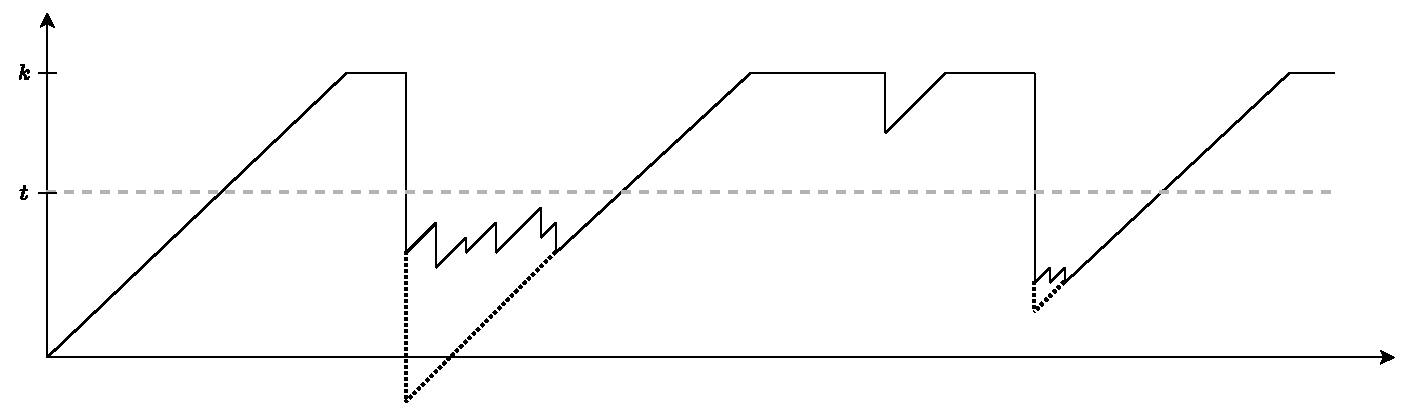
\includegraphics[width=1.0\linewidth]{fig/derandomized_MS.drawio.pdf}
    \caption{Derandomizing the MS vector. The y-axis is the length of a match ending at a given position in the query (the x-axis). The dashed horizontal line is the noise threshold. The dotted line shows the derandomized values. }
    \label{fig:derandomization}
\end{figure}

\begin{figure*}
    \centering
    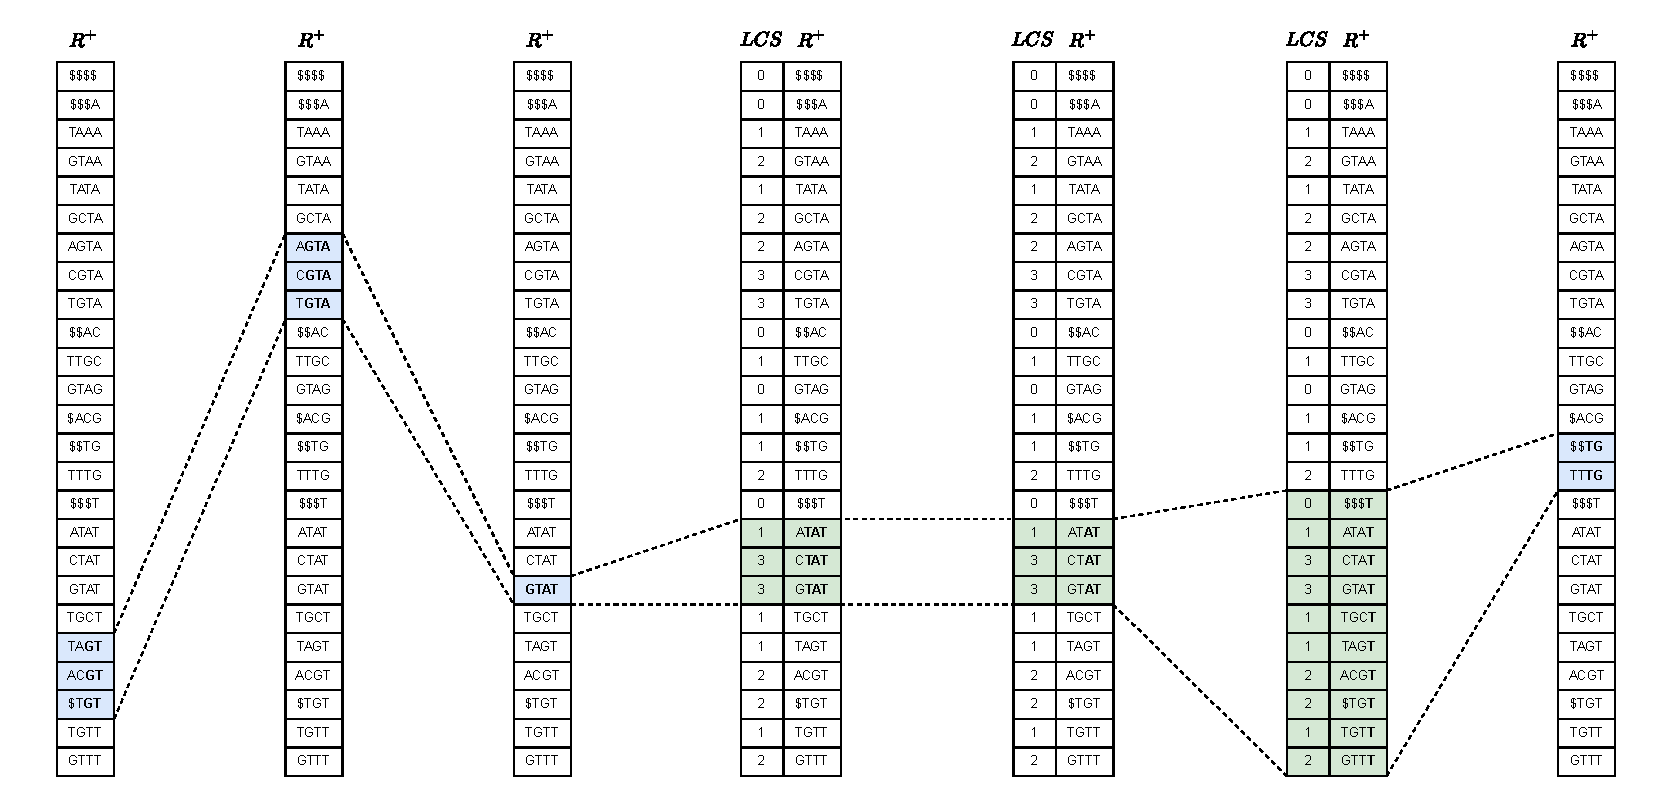
\includegraphics[scale=0.6]{fig/SBWT_search_LCS.drawio.pdf}
    \caption{Illustration of {\em ExtendRight} (resulting in blue intervals) and {\em ContractLeft} operations (resulting in green intervals) to match the string {\sf GTATG} with $k=4$ against a reference $\mathcal{S}= \{${\sf TGTTTG}, {\sf TTGCTAT}, {\sf ACGTAGTATAT}, {\sf TGTAAA}$\}$, $MS=\{ 1, 2, 3, 4, 2 \}$.\textcolor{red}{TODO:write derandomized MS, $DMS=\{1,2,3,4,2\}$? {\tt MMMRR}}}
    %\caption{ Illustration of three {\em ExtendRight} (resulting in blue intervals) and three {\em ContractLeft} operations (resulting in green intervals). GTATGTT\textcolor{red}{[TODO: maybe make a new example] }}
    \label{fig:sbwt-search}
\end{figure*}

%\subsection{\texorpdfstring{$k$-bounded matching statistics}{k-bounded matching statistics}}

The $k$-bounded matching statistics are defined as follows:

\begin{definition}\label{def:k-bounded-ms}
    ($k$-bounded matching statistics \cite{alanko2024finimizers})
    The $k$-bounded matching statistics for a query string $Q$ against a set of reference strings $S_1, \ldots, S_m$ is a vector $MS_k[1..|Q|]$ such that $MS_k[i]$ is the largest integer $l \leq k$ such that $Q[i-l+1..i]$ %\textcolor{red}{$Q[i..i-d+1]$ this is not a suffix ending in i}
    is a substring of at least one reference $S_1, \ldots, S_m$.
\end{definition}

In what follows, we may drop the subscript of $MS_k$ since $k$ is assumed constant throughout the paper.

The padded $k$-spectrum $R^+$ provides an equivalent and formulation that is easier to compute: the value of $MS[i]$ is the length $l$ of the longest \emph{suffix of a $k$-mer} in the padded spectrum of $T_1, \ldots, T_m$ that matches $Q[i-l+1..i]$. The $k$-mers in $R^+$ that have suffix $Q[i-l+1..i]$ are adjacent in the colexicographically sorted list of $k$-mers in $R^+$ (the colexicographic range of $Q[i-l+1..i]$). Algorithm \ref{alg:MS} shows pseudocode to compute the MS vector and the colexicographic ranges $[\ell, r]$ corresponding to the longest match at each position.

\begin{algorithm}
\begin{algorithmic}[1]
\small
\Require A query string $Q$ and a data structure supporting $ExtendRight$ and $ContractLeft$ on the padded $k$-mer spectrum. %in constant time. \\
\Ensure $MS_k[1..|Q|]$
\State $\ell, r \gets [1,n]$ \Comment{The current colexicographic range}
\State $l \gets 0$ \Comment{The length of the current match, up to $k$}
\State $MS_k[1..|Q|] \gets $ Array of length $|Q|$.
\For{$i = 1..|Q|$}
\While{$l > 0 \textbf{ and } ExtendRight(\ell, r, Q[i]) = \emptyset$}\label{line:MS-1-start}
    \State $\ell, r \gets ContractLeft(\ell, r)$
    \State $l \gets l-1$
\EndWhile \label{line:MS-1-end}
\If{$ExtendRight(\ell, r, Q[i]) \neq \emptyset$}
    \State $\ell, r \gets ExtendRight(\ell, r, Q[i])$\label{line:MS-2-start}
    \State $p \gets \min(k, l+1)$\label{line:MS-2-end}
\EndIf
\State $MS_k[i] \gets l$ %\Comment{The frequency of the match is $r - \ell + 1$} 
\label{line:MS-4-assignment}
\EndFor
\caption{\small $k$-bounded matching statistics.} 
\label{alg:MS}
\end{algorithmic}
\end{algorithm}

\subsection{Identifying statistically significant match positions}\label{sec:random-match-model}
For each query $Q$, we use Algorithm \ref{alg:MS} to compute the matching statistics vector $MS_k[1..|Q|]$. The matching statistic $MS_k[i]$ is the length of the longest match ending at position $i$ in $Q$, up to length $k$ (See Definition \ref{def:k-bounded-ms}). Even a random query will likely match some number of nucleotides at every position by chance alone. Our goal in this section is to derive a threshold for a statistically significant match length.

This threshold must be a function of the number of $k$-mers in the index: the larger the amount of indexed data, the longer matches we expect to find by chance. Let us denote the set of $k$-mers in the index with $\mathcal I$. We use a model where all the $k$-mers in $\mathcal I$ are independent random strings. The match length distribution at a given position against a single random $k$-mer follows a geometric distribution truncated at $k$. To simplify the formulas, we assume an untruncated geometric distribution. This is reasonable since for values $k \geq 30$ that we use, a full $k$-mer match is extremely unlikely. With these assumptions, if $X$ is the random variable denoting the length of the match against a single $k$-mer, the cumulative distribution $P(X \leq t)$ is given by:

\begin{equation}
    P\left(X \leq t\right) = 1 - p^{t + 1},
\label{geom-distribution}
\end{equation}
where $p$ is the probability that two nucleotides match by chance, e.g. $p = 1/4$. Now, let $M$ be a random variable denoting the length of the longest suffix match ending at some position $Q[i]$ against the entire index $\mathcal{I}$ containing $n$ distinct $k$-mers. Since the $k$-mers in $\mathcal I$ are assumed to be independent, the CDF of the maximum match length is:

%Since distribution of the longest common prefix of the query string $S_k$ and any string $S_i \in \mathcal{I}$ from the index $\mathcal{I}$ is given by the random variable $\mathcal{X}$, 
%we can define a new random variable $\mathcal{M}$ 
%which is the maximum of $n$ independent random variables with the same distribution as 
%$\mathcal{X}$ by setting 
%$\mathcal{M} = \text{max}\left\{\mathcal{X}_1, \text{\textellipsis}, \mathcal{X}_n\right\}$. 
%Because the variables $\mathcal{X}$ were assumed independent, the CDF of $\mathcal{M}$ is the product of $n$ random variables with the cumulative distribution function from Equation (\ref{geom-distribution})

\begin{equation}
    P\left(M \leq t\right) = P\left(X \leq t\right)^n = \left(1 - p^{t + 1}\right)^n
\label{max-of-geom-distributions}    
\end{equation}
Suppose we want to consider a match as statistically significant if it occurs with probability at most $r$ in our model. We can determine the corresponding match length $t_p$ by setting the CDF in Equation \ref{max-of-geom-distributions} to greater than $1-r$ and solving for $t$. We obtain:

\begin{equation}\label{analytic_noise_treshold}
t_p \geq \frac{\log (1 - (1-r)^{1/n})}{\log p} - 1\;,
\end{equation}
For example, for a small genome with $n = 10^6$ distinct $k$-mers,  nucleotide match probability $p = 0.25$ and false positive tolerance $r = 10^{-6}$, we have $t_p \approx 18.9$.

\subsection{\texorpdfstring{Derandomizing $k$-bounded matching statistic vectors}{Derandomizing k-bounded matching statistic vectors}}

Using the threshold $t_p$ from Equation (\ref{analytic_noise_treshold}), we \emph{derandomize} $MS_k$ by replacing match lengths below the threshold $t_p$ with values derived from nearby values. A key fact to understand about the $MS_k$ vector is that always $MS[i]$ at most $MS[i-1]+1$. For typical real data, the general shape of the $MS_k$ vector is a mountainscape with slow climbs and sharp falls, interspersed with with noisy valleys below the significant match threshold (see Figure \ref{fig:derandomization}). The idea of derandomization is to extrapolate the climbs backward to eliminate the noisy segments. The process is detailed in Algorithm \ref{alg:derandomized-MS}. After this processing, we can easily read off the lengths of gaps in the matches, as shown in the next section.

\begin{comment}
    version $d = d_1, \dots, d_N$ of the matching statistics vector $MS$ by iterating over $MS$ in reverse and applying the following procedure on the elements $MS[n] = ms_N, \dots, ms_1$
\begin{enumerate}
\item If $MS[n] > t_p$ and $MS[n+1] < MS[n]$,  then $d_n = MS[n]$,
\item If $MS[n] = k$, then $d_n = k$,
\item By default $d_n = MS[n+1] - 1$
\end{enumerate}
\end{comment}

%TODO ref to alg below



\begin{algorithm}
\begin{algorithmic}[1]
\small
\Require Matching statistics vector $MS_k[1..n]$, significant match threshold $t_p$ from Equation \ref{analytic_noise_treshold}.
\Ensure Derandomized MS vector $DMS_k[1..n] = (d_1, \ldots, d_{n})$.
\State $DMS_k[n] \gets MS_k[n]$
\For{$i = 1..n-1$ in reverse order}
\If{$MS_k[i] = k$}
\State $DMS_k[i] \gets k$
\ElsIf{$MS_k[i] \geq t_p$ and $MS[i+1] > MS[i]$}
    \State $DMS_k[i] \gets MS_k[i]$
\Else
    \State $DMS_k[i] \gets DMS_k[i+1]-1$
\EndIf
\EndFor
\caption{\small Derandomizing the MS vector} 
\label{alg:derandomized-MS}
\end{algorithmic}
\end{algorithm}

\subsection{Translating derandomized matching statistics into alignment events}

\begin{figure*}[!b]%
\centering
{\includesvg{Figure_translate_cases}}
\caption{\textbf{Draft Applying the translation procedure to a derandomized matching statistics vector.}. Panel a) shows the result of translating a single position at a time. Panel b) shows the result of translating an entire vector with multiple cases. Examples in both panels assume \emph{k}-mer size 3 and derandomization threshold 2.\textcolor{blue}{Would it be stupid to add MS here? (Elena)} \textcolor{red}{I think it's a good idea (Jarno)} \textcolor{blue}{I added a new figure below (Elena)} }\label{fig2}
\end{figure*}

\begin{figure*}[h!]
\small
    \centering
    
    % Table (a)
    \subfigure[\small Translating a single position at a time]{%
        \begin{tabular}{p{1.2cm} *{29}{p{.09cm}}}
\setlength{\extrarowheight}{-2pt} % Decrease row height
 & \multicolumn{6}{c}{\textbf{Only matches}} &  &  & \multicolumn{7}{c}{\textbf{Single mismatch}} &  &  &  \multicolumn{9}{c}{\textbf{Multiple deletions}} & \\
Reference & {\sf A} & {\sf C} & {\sf G} & {\sf C} & {\sf A} & {\sf G}  &  &  & {\sf A} & {\sf C} & {\sf G} & {\sf T} & {\sf C} & {\sf A} & {\sf G}  &  &  & {\sf A} & {\sf C} & {\sf G} & {\sf T} & {\sf T} & {\sf T} & {\sf C} & {\sf A} & {\sf G} &  &  \\
Query & {\sf A} & {\sf C} & {\sf G} & {\sf C} & {\sf A} & {\sf G}  &  &  & {\sf A} & {\sf C} & {\sf G} & {\sf C} & {\sf C} & {\sf A} & {\sf G}  &  &  & {\sf A} & {\sf C} & {\sf G} & {\tt -} & {\tt -} & {\tt -} & {\sf C} & {\sf A} & {\sf G} &  &  \\
$MS$ & 1 & 2 & 3 & 3 & 3 & 3 &   &  & 1 & 2 & 3 & 1 & 1 & 2 & 3 & & & 1 & 2 & 3 &  & &  & 1 & 2 & 3 &  &  &  \\
$DMS$ & 1 & 2 & 3 & 3 & 3 & 3 & & & 1 & 2 & 3 & 0 & 1 & 2 & 3 & & & 1 & 2 & 3 & & & & 1 & 2 & 3 &  &  &  \\
Output & {\tt M} & {\tt M} & {\tt M} & {\tt M} & {\tt M} & {\tt M} & & & {\tt M} & {\tt M} & {\tt M} & {\tt X} & {\tt M} & {\tt M} & {\tt M} & & & {\tt M} & {\tt M} & {\tt R}  & &  &  & {\tt R} & {\tt M} & {\tt M} &  &  &  \\
 \\
 & \multicolumn{7}{c}{\textbf{Single insertion}} &  & \multicolumn{8}{c}{\textbf{Multiple insertions}} &  & \multicolumn{12}{c}{\textbf{Recombination}} \\
Reference & {\sf A} & {\sf C} & {\sf G} & {\tt -} & {\sf C} & {\sf A} & {\sf G} &  & {\sf A} & {\sf C} & {\sf G} & {\tt -} & {\tt -} & {\sf C} & {\sf A} & {\sf G} &  & {\sf A} & {\sf C} & {\sf G} & {\sf T} & {\sf T} & {\sf T} & {\sf C} & {\sf G} & {\sf G} & {\sf C} & {\sf C} & {\sf C} \\
Query & {\sf A} & {\sf C} & {\sf G} & {\sf C} & {\sf C} & {\sf A} & {\sf G} &  & {\sf A} & {\sf C} & {\sf G} & {\sf T} & {\sf T} & {\sf C} & {\sf A} & {\sf G} &  & {\sf A} & {\sf C} & {\sf G} & {\sf C} & {\sf G} & {\sf G} & {\sf T} & {\sf T} & {\sf T} & {\sf C} & {\sf C} & {\sf C} \\
$MS$ & 1 & 2 & 3 & 3 & 1 & 2 & 3 &  & 1 & 2 & 3 & 0 & 0 & 1 & 2 & 3  &  & 1 & 2 & 3 & 2 & 2 & 3 & 2 & 3 & 3 & 3 & 2 & 3 \\
$DMS$ & 1 & 2 & 3 & 3 & 1 & 2 & 3 &  & 1 & 2 & 3 & \makebox[0.3cm]{\small -1} & 0 & 1 & 2 & 3 &  & 1 & 2 & 3 & 1 & 2 & 3 & 2 & 3 & 3 & 3 & 2 & 3 \\
Output & {\tt M} & {\tt M} & {\tt M} & {\tt X} & {\tt M} & {\tt M} & {\tt M} &  & {\tt M} & {\tt M} & {\tt M} & {\tt -} & {\tt -} & {\tt M} & {\tt M} & {\tt M} &  & {\tt M} & {\tt M} & {\tt R} & {\tt R} & {\tt M} & {\tt M} & {\tt M} & {\tt M} & {\tt R} & {\tt R} & {\tt M} & {\tt M} \\
\end{tabular}

    }
    \vspace{.5em} % Space between tables
    
    % Table (b)
    \subfigure[\small Translating an entire vector with multiple cases.]{%
        \begin{tabular}{p{1.2cm} *{20}{p{.09cm}}}
\setlength{\extrarowheight}{-2pt} % Decrease row height
\textbf{} & \multicolumn{20}{c}{\textbf{all cases in a single query}} \\
reference & {\sf A} & {\sf A} & {\sf A} & {\sf G} & {\sf A} & {\sf A} & {\sf C} & {\sf C} & {\sf A} & {\tt -} & {\sf T} & {\sf C} & {\sf A} & {\tt -} & {\tt -} & {\sf G} & {\sf G} & {\sf G} & {\sf C} & {\sf G} \\
query & {\sf C} & {\sf A} & {\sf A} & {\sf G} & {\tt -} & {\tt -} & {\sf C} & {\sf C} & {\sf A} & {\sf C} & {\sf T} & {\sf C} & {\sf A} & {\sf T} & {\sf T} & {\sf G} & {\sf G} & {\sf G} & {\sf T} & {\sf C} \\
MS & 0 & 2 & 2 & 3 &  &  & 2 & 2 & 3 & 2 & 1 & 2 & 3 & 3 & 1 & 1 & 2 & 3 & 1 & 2 \\
dMS & 0 & 1 & 2 & 3 &  &  & 1 & 2 & 3 & 0 & 1 & 2 & 3 & \makebox[0.3cm]{\small -1} & 0 & 1 & 2 & 3 & \textbf{\makebox[0.3cm]{\small -1}} & \textbf{0} \\
output & {\tt X} & {\tt M} & {\tt M} & {\tt R} & {\sf } & {\sf } & {\tt R} & {\tt M} & {\tt M} & {\tt X} & {\tt M} & {\tt M} & {\tt M} & {\tt -} & {\tt -} & {\tt M} & {\tt M} & {\tt M} & {\tt -} & {\tt -}
\end{tabular}
    }
    \caption{Illustration of the results of applying the translation procedure to a derandomized matching statistics vector. Examples in both panels assume \emph{k}-mer size 3 and derandomization threshold $t=2$. \textcolor{blue}{Elena: I would remove the row "position"}}
    \label{fig:translate_cases}
\end{figure*}

%Zeros in $d$ mark the first base after end of a match, and negative values denote 0-indexed distance from the last matching base. The key to this simple procedure is reading the matching statistics vector $MS$ in reverse and using the threshold $t_p$ to determine when a new match begins after a gap.


The derandomized MS vector can be translated into a character representation of the compatibility between the query and a reference sequence. For example, a single nucleotide substitution or insertion at position $i$ will show up as run from 0 to $k$ in $DMS_k[i..i+k]$. These can be distinguished from deletions and recombinations, which exhibit different kinds of characteristic patterns. All the possible cases are displayed in Figure \ref{fig:translate_cases}a. We represent character compatibility events using the following set of symbols:

\begin{enumerate}
\item[\textbf{$\tt{M}$}]: Match between query and reference.
\item[\textbf{-}]: Bases in the query that are not found in the reference.
\item[\textbf{$\tt{X}$}]: Single base mismatch \textit{or} single base insertion into the query.
\item[\textbf{$\tt{R}$}]: Two consecutive ${\tt R}$s signify a discontinuity in the alignment. The right ${\tt R}$ is at the start of a $k$-mer that is not adjacent to the last character in the $k$-mer corresponding to the left ${\tt R}$. This implies either a deletion of unknown length in the query, or an insertion of $k$-mers from elsewhere in the reference into the query.
\end{enumerate}
Algorithm \ref{alg:tranlating-DMS} shows how these events can be detected with a single backward pass over the $DMS_k$ array. Figure \ref{fig:translate_cases}b shows an example where all the cases occur in a single query. Note how this example illustrates that the procedure is not able to distinguish between a single base insertion and a single base substitution. This problem can be resolved by adding a \textit{refinement} step to our translation, which resolves this conundrum by using the nucleotide sequence of the reference.


%Applying the translation procedure over a more complex derandomized MS vector with multiple events is illustrated in Figure \ref{fig:translate_cases}b. 
%The translation $T$ for each value in the derandomized MS vector depends on the neighboring values and the threshold $t_p$. We use the following algorithm to determine the character representation of the events.

\begin{algorithm}
\begin{algorithmic}[1]
\small
\Require Derandomized Matching statistics vector $DMS_k[1..n]$, significant match threshold $t_p$ from Equation \ref{analytic_noise_treshold}. We assume the sentinel values $DMS_k[0] = k$ and $DMS_k[n+1] = DMS_k[n]$.
\Ensure $T$, Tranlated DMS vector.%$DMS_k[1..|Q|] = (d_1, \ldots, d_{|Q|})$.
\State $T \leftarrow $ Array of length $n$ initialized to ' '
\For{$i = 1..n$}
%if !(pos > 1 && res[pos - 1] == 'R' && res[pos] == 'R') {
\If{$T[i] \neq {\tt R}$}
\If{$DMS_k[i] > t_p$ and $0 < DMS_k[i+1] < t_p$ }
\State $T[i] = {\tt R}$
\State $T[i+1] = {\tt R}$ 
\ElsIf{$DMS_k[i] \leq 0$} \Comment{Mismatch}
    \If{ $DMS_k[i+1] = 1$ and $DMS_k[i-1] > 0$ }
    \State $T[i] \gets {\tt X}$
    \Else
    \State $T[i] \gets {\tt -}$
    \EndIf
\Else
    \State $T[i] = {\tt M}$ \Comment{Match}
\EndIf
\EndIf
\EndFor
%\State \Return $T$
\caption{\small Translating the DMS vector} 
\label{alg:tranlating-DMS}
\end{algorithmic}
\end{algorithm}

\begin{comment}
The translation $t_n$ for each value in the derandomized MS vector $d_n$ depends on the neighboring values $d_{n - 1}$, $d_{n + 1}$ and the threshold $t_p$. We use the following algorithm to determine the character representation of the events
    \begin{enumerate}
\item If $d_n > t_p$ and $d_{n + 1} > 0$ and $d_{n + 1} < t_p$, \\ then $t_n = \text{'R'}$ and $t_{n + 1} = \text{'R'}$.
\item If $d_n <= 0$, then there is a mismatch in the query and we apply
    \begin{enumerate}
    \item If $d_{n + 1} = 1$ and $d_{n - 1} > 0$, then $t_n = \text{{\tt X}}$.
    \item Else $t_n = \text{'-'}$.
    \end{enumerate}
\item By default $t_n = \text{'M'}$
\end{enumerate}
\end{comment}





%\textcolor{red}{Here we would also like to refer the reader to the documentation for the "translate\_ms\_vec" and "translate\_ms\_val" functions in the translate module \footnote{https://docs.rs/kbo} for the actual implementation of these algorithms.}

\subsection{Refining the translation to resolve SNPs versus insertions}
\textcolor{red}{TODO this needs a description of how the base is deemed as a SNP (substitution?) or an insertion in the first place. Written below but to be checked...} \textcolor{blue}{The pseudocode in Algorithm \ref{alg:tranlating-DMS} now defines this}.
In kbo's output {\tt X} may represent either a single base substitution or a single base insertion.
A substitution indicates a mismatch between the base in the query and the base in the reference. In contrast, an insertion signifies that a single base is present in the query but absent in the reference; consequently, in the alignment, this base in the query aligns with a gap in the reference.
  
We can resolve the problem of single nucleotide substitution versus an insertion by using the LCS array \cite{alanko2023longest}. Briefly, this data structure allows retrieving the neighboring bases from the SBWT (in the colexicographical ordering) and provides an educated guess for the value of the base marked with an {\tt X}. The SBWT by itself does not store the original sequence, but the LCS array allows us to derive a workaround.

We resolve the {\tt X}s by checking whether the \emph{k}-mer whose first character overlaps the {\tt X} has a matching statistic of $k - 1$ and, if it does, traversing the colexicographical ordering until we find the \emph{k}-mer where the position marked by {\tt X} is the middle base (a split \emph{k}-mer centered on {\tt X} \cite{derelle2024seamless}). We use the middle base from this \emph{k}-mer to replace the {\tt X} in the translation. If the matching statistic is less than $k - 1$, the character is checked from the \emph{k}-mer that is $(t_p + 1)/2$ characters away from the {\tt X} to account for the possibility of a random match.

Although the colexicographical ordering is not guaranteed to return the exact \emph{k}-mer that is present in the query at this position, in practice the approach selects the same nucleotide as Snippy and SKA with a high probability (\textcolor{red}{TODO add figure from a simple example}).

\section{Use cases}

\subsection{Reference-based alignment of query assemblies with 'kbo map'}

Our algorithm can perform reference-based alignment, where the nucleotides in a query sequence are mapped relative to a reference sequence, by applying the full 'Map' pipeline from Fig. \ref{fig1}. When the pipeline is applied to multiple closely related query sequences against the same reference, this results in a "SNP alignment" that approximates multiple sequence alignment required in, for example, phylogenetic analyses but is much faster to obtain. To test 'kbo map' in a realistic use case, we benchmarked the runtime of 'kbo map' on obtaining SNP alignments and compared the results to two widely used bacterial genomics tools, ska2~\cite{derelle2024seamless, harris2018SKA} and snippy~\cite{seemann2015snippy}.



\textcolor{red}{TODO push experiment code and plotting code to \url{https://github.com/tmaklin/kbo-paper} and sync the repo to Zenodo for archival}

Specific to alignment

- alignments are comparable to Snippy and SKA map

- alignment is faster than Snippy or SKA map

- alignment scales easily to 10s of thousands of genomes.

- compare w/ Snippy, SKA map

\subsection{Finding reference gene sequences in a query assembly with 'kbo find'}

Specific to  find

- Quick if it's not needed to know which genes exactly are present

- Slower if the gene names (= individual contigs are needed). this could be implemented more efficiently with colors.

- compare w/ blast

\subsection{Running kbo in the browser}
- efficient resource use: no prebuilt indexes, no temporary space, low memory consumption, runs ok on a single thread

Available online \footnote{https://maklin.fi/kbo}.

\subsection{Browser queries for AllTheBacteria genomes}
- \textcolor{purple}{Let's save this for a separate project, it's too much to implement right now /TM}

- \textcolor{red}{TODO check feasibility of using some served genomes as the query or the target.}

\noindent- \textcolor{red}{TODO  make this available as an application for the AllTheBacteria project.}


\section{Discussion}
In no particular order:

- Adding colors: matching statistics queries

- index compression via pangenomes or colorset compression: we can compress ~45 000 genomes from the same species into a few gigabytes using the meta-diff indedx in Fulgor, implementing this in SBWT with efficient MS queries would enable simultaneous alignment against tens of thousands of genomes.

- possibilities for gene variant calling with colors

- finimizers: these together with the recombination markers output by {\sf kbo} (RR) could be used to identify potential recombination segments. Finimizers might additionally allow even more efficient queries with a prebuilt index?

- Mention how the webassembly version enables implementing tools like amrfinder, kaptive, and tree inference in the browser. Use the pks island gene typing as an example of how the custom database inclusion can be utilised.

\section{Code availability}
The Rust\footnote{\url{https://www.rust-lang.org/}} library, command-line interface, and graphical user interface implementing the methods described here are freely available from Codeberg \url{https://codeberg.org/themaklin/sablast} and GitHub \url{https://github.com/tmaklin/kbo} under a MIT\footnote{\url{https://opensource.org/license/mit}} and Apache 2.0\footnote{\url{https://www.apache.org/licenses/LICENSE-2.0}} dual license.

\section{Competing interests}
No competing interest is declared.

\section{Author contributions statement}
T.M. designed the kbo algorithms and implemented the kbo, kbo-cli, and kbo-gui Rust libraries. J.N.A. implemented the sbwt Rust crate and derived the random match distribution. T.M., J.N.A, E.B., and S.J.P. investigated the relationship between \emph{k}-bounded matching statistics and local alignments. S.J.P. obtained funding and supervised the study. All authors contributed to the writing, reviewing, and editing of the manuscript.

\section{Acknowledgments}
This work was supported in part by the Research Council of Finland via grant 351150. TM was supported by the Research Council of Finland (EuroHPC grant).

%\begin{tabular}{p{1.2cm} *{29}{p{.09cm}}}
\setlength{\extrarowheight}{-2pt} % Decrease row height
 & \multicolumn{6}{c}{\textbf{Only matches}} &  &  & \multicolumn{7}{c}{\textbf{Single mismatch}} &  &  &  \multicolumn{9}{c}{\textbf{Multiple deletions}} & \\
Reference & {\sf A} & {\sf C} & {\sf G} & {\sf C} & {\sf A} & {\sf G}  &  &  & {\sf A} & {\sf C} & {\sf G} & {\sf T} & {\sf C} & {\sf A} & {\sf G}  &  &  & {\sf A} & {\sf C} & {\sf G} & {\sf T} & {\sf T} & {\sf T} & {\sf C} & {\sf A} & {\sf G} &  &  \\
Query & {\sf A} & {\sf C} & {\sf G} & {\sf C} & {\sf A} & {\sf G}  &  &  & {\sf A} & {\sf C} & {\sf G} & {\sf C} & {\sf C} & {\sf A} & {\sf G}  &  &  & {\sf A} & {\sf C} & {\sf G} & {\tt -} & {\tt -} & {\tt -} & {\sf C} & {\sf A} & {\sf G} &  &  \\
$MS$ & 1 & 2 & 3 & 3 & 3 & 3 &   &  & 1 & 2 & 3 & 1 & 1 & 2 & 3 & & & 1 & 2 & 3 &  & &  & 1 & 2 & 3 &  &  &  \\
$DMS$ & 1 & 2 & 3 & 3 & 3 & 3 & & & 1 & 2 & 3 & 0 & 1 & 2 & 3 & & & 1 & 2 & 3 & & & & 1 & 2 & 3 &  &  &  \\
Output & {\tt M} & {\tt M} & {\tt M} & {\tt M} & {\tt M} & {\tt M} & & & {\tt M} & {\tt M} & {\tt M} & {\tt X} & {\tt M} & {\tt M} & {\tt M} & & & {\tt M} & {\tt M} & {\tt R}  & &  &  & {\tt R} & {\tt M} & {\tt M} &  &  &  \\
 \\
 & \multicolumn{7}{c}{\textbf{Single insertion}} &  & \multicolumn{8}{c}{\textbf{Multiple insertions}} &  & \multicolumn{12}{c}{\textbf{Recombination}} \\
Reference & {\sf A} & {\sf C} & {\sf G} & {\tt -} & {\sf C} & {\sf A} & {\sf G} &  & {\sf A} & {\sf C} & {\sf G} & {\tt -} & {\tt -} & {\sf C} & {\sf A} & {\sf G} &  & {\sf A} & {\sf C} & {\sf G} & {\sf T} & {\sf T} & {\sf T} & {\sf C} & {\sf G} & {\sf G} & {\sf C} & {\sf C} & {\sf C} \\
Query & {\sf A} & {\sf C} & {\sf G} & {\sf C} & {\sf C} & {\sf A} & {\sf G} &  & {\sf A} & {\sf C} & {\sf G} & {\sf T} & {\sf T} & {\sf C} & {\sf A} & {\sf G} &  & {\sf A} & {\sf C} & {\sf G} & {\sf C} & {\sf G} & {\sf G} & {\sf T} & {\sf T} & {\sf T} & {\sf C} & {\sf C} & {\sf C} \\
$MS$ & 1 & 2 & 3 & 3 & 1 & 2 & 3 &  & 1 & 2 & 3 & 0 & 0 & 1 & 2 & 3  &  & 1 & 2 & 3 & 2 & 2 & 3 & 2 & 3 & 3 & 3 & 2 & 3 \\
$DMS$ & 1 & 2 & 3 & 3 & 1 & 2 & 3 &  & 1 & 2 & 3 & \makebox[0.3cm]{\small -1} & 0 & 1 & 2 & 3 &  & 1 & 2 & 3 & 1 & 2 & 3 & 2 & 3 & 3 & 3 & 2 & 3 \\
Output & {\tt M} & {\tt M} & {\tt M} & {\tt X} & {\tt M} & {\tt M} & {\tt M} &  & {\tt M} & {\tt M} & {\tt M} & {\tt -} & {\tt -} & {\tt M} & {\tt M} & {\tt M} &  & {\tt M} & {\tt M} & {\tt R} & {\tt R} & {\tt M} & {\tt M} & {\tt M} & {\tt M} & {\tt R} & {\tt R} & {\tt M} & {\tt M} \\
\end{tabular}

%\begin{tabular}{p{1.2cm} *{20}{p{.09cm}}}
\setlength{\extrarowheight}{-2pt} % Decrease row height
\textbf{} & \multicolumn{20}{c}{\textbf{all cases in a single query}} \\
reference & {\sf A} & {\sf A} & {\sf A} & {\sf G} & {\sf A} & {\sf A} & {\sf C} & {\sf C} & {\sf A} & {\tt -} & {\sf T} & {\sf C} & {\sf A} & {\tt -} & {\tt -} & {\sf G} & {\sf G} & {\sf G} & {\sf C} & {\sf G} \\
query & {\sf C} & {\sf A} & {\sf A} & {\sf G} & {\tt -} & {\tt -} & {\sf C} & {\sf C} & {\sf A} & {\sf C} & {\sf T} & {\sf C} & {\sf A} & {\sf T} & {\sf T} & {\sf G} & {\sf G} & {\sf G} & {\sf T} & {\sf C} \\
MS & 0 & 2 & 2 & 3 &  &  & 2 & 2 & 3 & 2 & 1 & 2 & 3 & 3 & 1 & 1 & 2 & 3 & 1 & 2 \\
dMS & 0 & 1 & 2 & 3 &  &  & 1 & 2 & 3 & 0 & 1 & 2 & 3 & \makebox[0.3cm]{\small -1} & 0 & 1 & 2 & 3 & \textbf{\makebox[0.3cm]{\small -1}} & \textbf{0} \\
output & {\tt X} & {\tt M} & {\tt M} & {\tt R} & {\sf } & {\sf } & {\tt R} & {\tt M} & {\tt M} & {\tt X} & {\tt M} & {\tt M} & {\tt M} & {\tt -} & {\tt -} & {\tt M} & {\tt M} & {\tt M} & {\tt -} & {\tt -}
\end{tabular}


\bibliographystyle{plain}
\bibliography{reference}


%USE THE BELOW OPTIONS IN CASE YOU NEED AUTHOR YEAR FORMAT.
%\bibliographystyle{abbrvnat}
%\bibliography{reference}

\end{document}
